\chapter{The Energy of Reactions: Combustion and Bond Energies}\label{ch:g11:reaction-energy}

Break the seal of a hand warmer and, a minute later, it is too hot to
hold for long; squeeze a cold pack and it chills a sprained ankle; a city
bus runs all day on hydrogen and leaves only water vapour behind it.
Chemical transformations do not only turn substances into others: they
release energy, or take it in. Where does that energy come from, and how
much of it can a \omterm{def:g4:what-a-fire-needs:fuel}{fuel} give?

\begin{recall}
In a \omterm{def:g8:combustion-and-fuels:complete}{complete combustion}, a \omterm{def:g4:what-a-fire-needs:fuel}{fuel} made of carbon and hydrogen burns in
dioxygen to give carbon dioxide and water
(\cref{ch:g8:combustion-and-fuels}). A \omterm{def:g10:lewis-and-shape:covalent-bond}{covalent bond} is a shared pair of
\omterm{def:g9:inside-the-atom:nucleus}{electrons}; \omterm{def:g10:lewis-and-shape:lewis-structure}{Lewis structures} show every bond of a \omterm{def:g7:atoms-and-molecules:molecule}{molecule}
(\cref{ch:g10:lewis-and-shape}). The \omterm{def:g10:the-mole:amount}{amount of substance} is counted in
\omterm{def:g10:the-mole:amount}{moles} (\cref{ch:g10:the-mole}).
\end{recall}

\begin{omfigure}
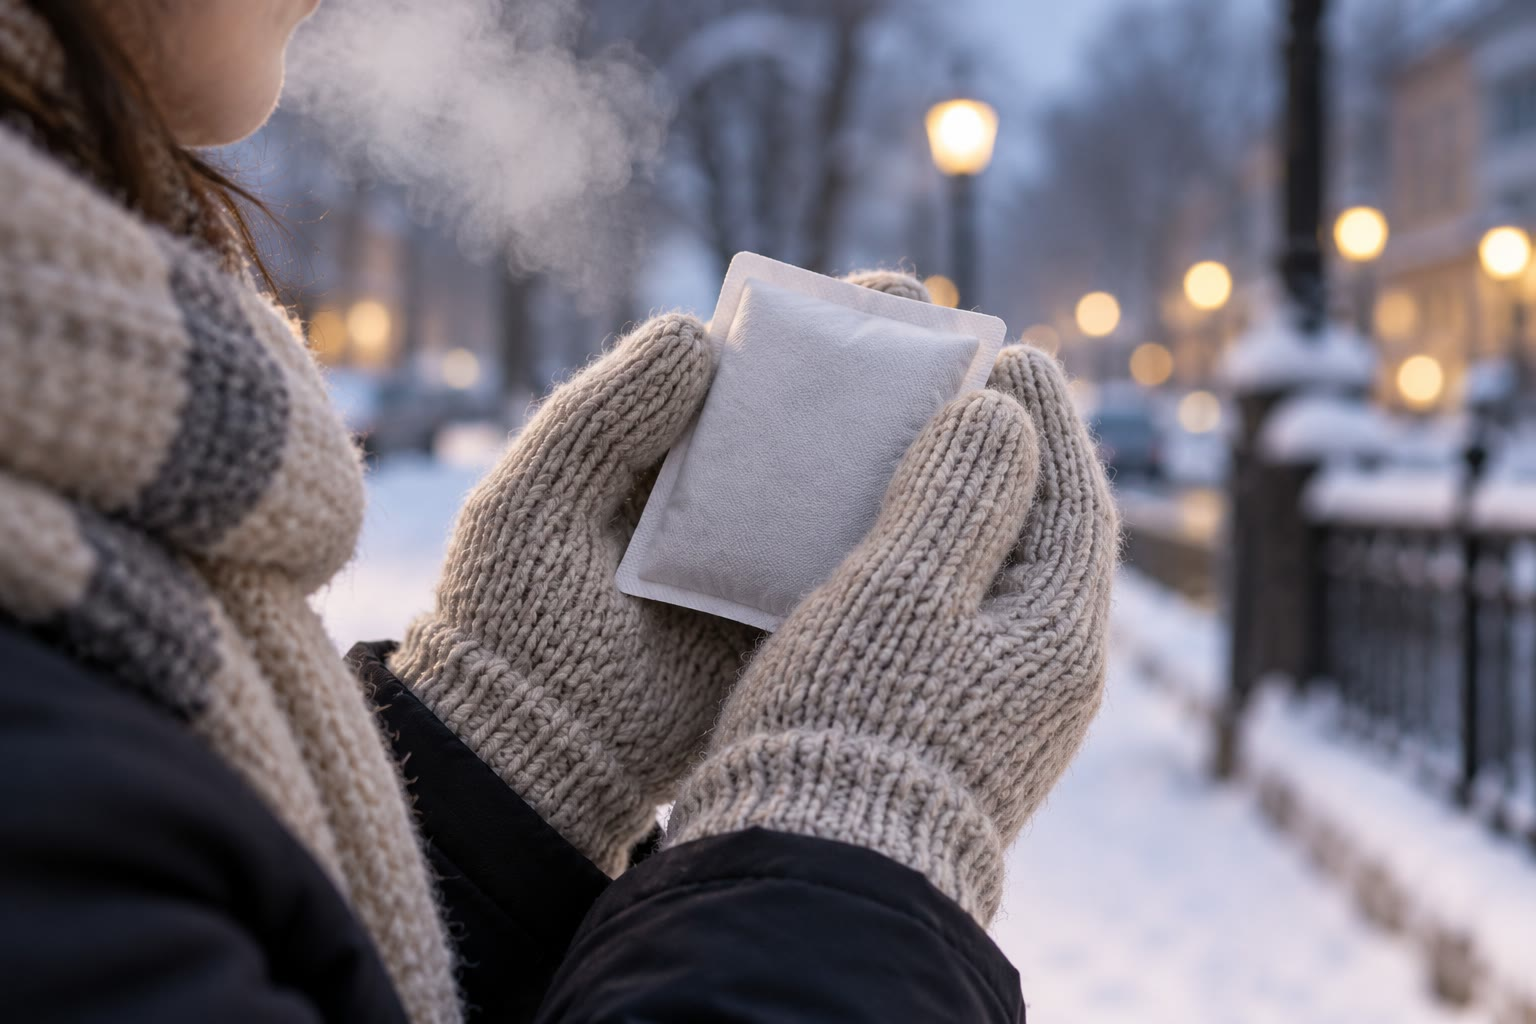
\includegraphics[width=0.45\linewidth]{images/book1/ai/g11-hand-warmers.jpg}

{\small A hand warmer: a reaction inside the pouch releases heat.}
\end{omfigure}

\section{Exothermic and endothermic transformations}

\begin{definition}[Exothermic, endothermic]\label{def:g11:reaction-energy:exothermic}
A transformation is \emph{exothermic}\index{exothermic} if it releases
energy to its surroundings, usually as heat: the surroundings warm up.
It is \emph{endothermic}\index{endothermic} if it takes in energy from
its surroundings: they cool down, or the transformation needs heating to
go on.
\end{definition}

\begin{example}[Warm and cold]\label{ex:g11:reaction-energy:packs}
\omterm{def:g4:what-a-fire-needs:burning}{Combustions} are \omterm{def:g11:reaction-energy:exothermic}{exothermic}, and so is the slow reaction of iron powder
with the dioxygen of the \omterm{def:g4:air-a-mixture-of-gases:air}{air} inside a hand warmer. The dissolving of
ammonium nitrate in water, used in cold packs, is \omterm{def:g11:reaction-energy:exothermic}{endothermic}; so is the
decomposition of limestone into quicklime and carbon dioxide, which
takes place only in a very hot kiln.
\end{example}

\begin{omfigure}
\begin{tikzpicture}[font=\small]
  \begin{scope}
    \draw[->] (0,0) -- (0,3.2) node[above] {energy};
    \draw[very thick, omDef] (0.5,2.5) -- (2.3,2.5) node[right, text=black] {reactants};
    \draw[very thick, omProp] (0.5,0.8) -- (2.3,0.8) node[right, text=black] {products};
    \draw[->, thick, omThm] (1.4,2.45) -- (1.4,0.85);
    \node[omThm, anchor=west, align=left] at (1.5,1.65) {energy\\ released};
    \node[anchor=north] at (1.6,-0.15) {\textbf{exothermic}};
  \end{scope}
  \begin{scope}[xshift=6cm]
    \draw[->] (0,0) -- (0,3.2) node[above] {energy};
    \draw[very thick, omDef] (0.5,0.8) -- (2.3,0.8) node[right, text=black] {reactants};
    \draw[very thick, omProp] (0.5,2.5) -- (2.3,2.5) node[right, text=black] {products};
    \draw[->, thick, omDef] (1.4,0.85) -- (1.4,2.45);
    \node[omDef, anchor=west, align=left] at (1.5,1.65) {energy\\ taken in};
    \node[anchor=north] at (1.6,-0.15) {\textbf{endothermic}};
  \end{scope}
\end{tikzpicture}

{\small Energy diagrams. In an \omterm{def:g11:reaction-energy:exothermic}{exothermic} reaction the products hold less
energy than the \omterm{def:g7:chemical-reactions:reactant}{reactants}, and the difference is released; in an
\omterm{def:g11:reaction-energy:exothermic}{endothermic} one they hold more, and it must be supplied.}
\end{omfigure}

\section{The energy released by a combustion}

\begin{definition}[Molar energy of combustion]\label{def:g11:reaction-energy:combustion-energy}
The \emph{molar energy of combustion}\index{molar energy of combustion}
$E_c$ of a \omterm{def:g4:what-a-fire-needs:fuel}{fuel} is the energy released by the \omterm{def:g8:combustion-and-fuels:complete}{complete combustion} of one
\omterm{def:g10:the-mole:amount}{mole} of it, in \si{kJ/mol}, the water formed being liquid.
\end{definition}

\begin{proposition}[Energy released by $n$ moles]\label{prop:g11:reaction-energy:n-moles}
% ledger: dch:CH4
The \omterm{def:g8:combustion-and-fuels:complete}{complete combustion} of an amount $n$ of \omterm{def:g4:what-a-fire-needs:fuel}{fuel} releases the energy
$Q = n \times E_c$. For methane, $E_c = \qty{890.7}{kJ/mol}$: \omterm{def:g4:what-a-fire-needs:burning}{burning}
\qty{1.00}{mol} (\qty{16.0}{g}) of it releases about \qty{891}{kJ}.
\end{proposition}

\begin{proof}
Each \omterm{def:g10:the-mole:amount}{mole} of \omterm{def:g4:what-a-fire-needs:fuel}{fuel} burnt releases $E_c$; $n$ \omterm{def:g10:the-mole:amount}{moles} release $n$ times
more.
\end{proof}

\begin{inthelab}[Heating water with a spirit burner]
% ledger: cp:water
A spirit burner of ethanol is weighed, then lit under a \omterm{def:g9:periodic-table-first-look:metal}{metal} can holding
\qty{200}{g} of water, with a thermometer in it. When the water has
warmed by \qty{25}{\celsius}, the flame is put out and the burner
weighed again: it has lost \qty{1.50}{g} of ethanol. The energy taken by
the water is computed with the physics formula $Q = m\, c\, \Delta\theta$,
where $c = \qty{4.18}{J/(g.\celsius)}$ is the specific heat of water. It
is far below the energy the ethanol could release: much of the heat
warms the \omterm{def:g4:air-a-mixture-of-gases:air}{air}, the can and the burner, and some of the ethanol burns
incompletely.
\end{inthelab}

\begin{omfigure}
\begin{tikzpicture}[font=\small]
  % spirit burner
  \fill[black!8, draw=black!60] (-0.6,0) rectangle (0.6,0.7);
  \fill[cyan!15] (-0.55,0.05) rectangle (0.55,0.45);
  \fill[black!40] (-0.06,0.7) rectangle (0.06,0.95);
  \fill[orange!70!yellow] (0,0.95) .. controls (-0.25,1.25) and (-0.1,1.6) .. (0,1.85)
    .. controls (0.1,1.6) and (0.25,1.25) .. (0,0.95);
  \fill[yellow!40] (0,1.0) .. controls (-0.1,1.2) and (-0.05,1.4) .. (0,1.5)
    .. controls (0.05,1.4) and (0.1,1.2) .. (0,1.0);
  % tripod and can
  \draw[black!60, line width=1pt] (-1.1,0) -- (-0.9,2.1) (1.1,0) -- (0.9,2.1);
  \draw[black!60, line width=1.2pt] (-1.1,2.1) -- (1.1,2.1);
  \fill[black!15, draw=black!60] (-0.8,2.1) rectangle (0.8,3.7);
  \fill[omWater] (-0.75,2.15) rectangle (0.75,3.3);
  % thermometer
  \pic at (0.35,2.35) {thermometer};
  \draw[omProp, thick, <-] (0.6,0.35) -- (2.0,0.35) node[right, text=black]
    {spirit burner (ethanol)};
  \draw[omProp, thick, <-] (0.8,2.9) -- (2.0,2.9) node[right, text=black]
    {can: \qty{200}{g} of water};
  \draw[omProp, thick, <-] (0.45,5.0) -- (2.0,5.0) node[right, text=black]
    {thermometer};
\end{tikzpicture}

{\small Measuring the energy given by a \omterm{def:g4:what-a-fire-needs:fuel}{fuel}: a spirit burner heats a can
of water whose temperature rise is measured.}
\end{omfigure}


\begin{example}[The spirit burner in numbers]\label{ex:g11:reaction-energy:burner}
% ledger: cp:water, dch:C2H5OH, aw:C, aw:H, aw:O
The water received $Q = 200 \times 4.18 \times 25 = \qty{2.09e4}{J}$,
that is \qty{20.9}{kJ}. The ethanol burnt, \qty{1.50}{g}, is
$1.50 / 46.0 = \qty{0.0326}{mol}$; with $E_c = \qty{1367.6}{kJ/mol}$ it
could release $0.0326 \times 1367.6 = \qty{44.6}{kJ}$. Only
$20.9 / 44.6 \approx \qty{47}{\percent}$ of it reached the water.
\end{example}

\section{Bond energies}

\begin{definition}[Bond energy]\label{def:g11:reaction-energy:bond-energy}
The \emph{bond energy}\index{bond energy} of a \omterm{def:g10:lewis-and-shape:covalent-bond}{covalent bond} is the energy
needed to break one \omterm{def:g10:the-mole:amount}{mole} of such bonds, the \omterm{def:g7:atoms-and-molecules:molecule}{molecules} and \omterm{def:g7:atoms-and-molecules:atom}{atoms} being
gases. Tables give average values, measured over many \omterm{def:g7:atoms-and-molecules:molecule}{molecules}, in
\si{kJ/mol}.
\end{definition}

\begin{omfigure}
\small
% ledger: be:H-H, be:C-H, be:N-H, be:O-H, be:H-Cl, be:C-C, be:CC-double, be:C-O, be:CO-double, be:NN-triple, be:OO-double, be:Cl-Cl
\begin{tabular}{lr@{\qquad}lr@{\qquad}lr}
\hline
bond & \si{kJ/mol} & bond & \si{kJ/mol} & bond & \si{kJ/mol} \\
\hline
\ce{H-H} & 436 & \ce{C-C} & 345 & \ce{O=O} & 498 \\
\ce{C-H} & 415 & \ce{C=C} & 611 & \ce{N#N} & 946 \\
\ce{N-H} & 390 & \ce{C-O} & 350 & \ce{Cl-Cl} & 243 \\
\ce{O-H} & 464 & \ce{C=O} & 741 & \ce{H-Cl} & 432 \\
\hline
\end{tabular}\par\medskip

{\small Average bond energies. Breaking a bond always costs energy;
forming it gives the same energy back.}
\end{omfigure}

\begin{omfigure}
\begin{tikzpicture}[font=\small, x=1cm, y=0.0015cm]
  \draw[->] (0,-850) -- (0,2900) node[above] {energy (\si{kJ})};
  \draw[very thick, black!60] (0.4,2656) -- (3.9,2656);
  \node[anchor=west] at (4.0,2656) {separate atoms: \ce{C + 4H + 4O}};
  \draw[very thick, omDef] (0.4,0) -- (3.9,0);
  \node[anchor=west] at (4.0,0) {\ce{CH4 + 2O2}};
  \draw[very thick, omProp] (0.4,-682) -- (3.9,-682);
  \node[anchor=west] at (4.0,-682) {\ce{CO2 + 2H2O}};
  \draw[->, thick, omDef] (1.0,30) -- (1.0,2626);
  \node[omDef, anchor=west, align=left] at (1.05,1500) {break 4 \ce{C-H}\\ and 2 \ce{O=O}:\\ $+\qty{2656}{kJ}$};
  \draw[->, thick, omProp] (3.4,2626) -- (3.4,-652);
  \node[omProp, anchor=west, align=left] at (3.45,1200) {form 2 \ce{C=O}\\ and 4 \ce{O-H}:\\ $-\qty{3338}{kJ}$};
  \draw[<->, omThm, thick] (0.6,-10) -- (0.6,-672);
  \node[omThm, anchor=west] at (0.65,-341) {$E_r \approx \qty{-682}{kJ}$};
\end{tikzpicture}

{\small The \omterm{def:g4:what-a-fire-needs:burning}{combustion} of methane as two imaginary steps, with average
bond energies: breaking every bond, then forming the new ones. The
estimate, \qty{-682}{kJ} per \omterm{def:g10:the-mole:amount}{mole} of methane, is \omterm{def:g11:reaction-energy:exothermic}{exothermic}.}
\end{omfigure}

\begin{proposition}[Estimating a reaction energy]\label{prop:g11:reaction-energy:estimate}
For a reaction between gases, the energy taken in, $E_r$ (negative if
energy is released), is approximately
\[
  E_r \approx \sum E(\text{bonds broken}) - \sum E(\text{bonds formed}) .
\]
If $E_r < 0$, more energy is released by forming the new bonds than is
needed to break the old ones: the reaction is \omterm{def:g11:reaction-energy:exothermic}{exothermic}.
\end{proposition}

\begin{proof}
Imagine the reaction in two steps: every bond of the \omterm{def:g7:chemical-reactions:reactant}{reactants} is broken,
which costs the first sum and leaves separate \omterm{def:g7:atoms-and-molecules:atom}{atoms}; then the bonds of
the products form, which gives back the second sum. The result is only an
estimate, because tables give averages over many \omterm{def:g7:atoms-and-molecules:molecule}{molecules}.
\end{proof}

\begin{method}[Estimating a reaction energy from bond energies]\label{met:g11:reaction-energy:bonds}
\begin{enumerate}
  \item Write the \omterm{def:g8:balanced-equations:equation}{balanced equation} and the \omterm{def:g10:lewis-and-shape:lewis-structure}{Lewis structure} of every
        \omterm{def:g7:atoms-and-molecules:molecule}{molecule}.
  \item Count the bonds of each kind broken in the \omterm{def:g7:chemical-reactions:reactant}{reactants} and formed
        in the products, with the coefficients.
  \item Add up the energies of the bonds broken, subtract those of the
        bonds formed.
  \item Conclude: a negative result means an \omterm{def:g11:reaction-energy:exothermic}{exothermic} reaction.
\end{enumerate}
\end{method}

\begin{example}[Hydrogen and chlorine]\label{ex:g11:reaction-energy:hcl}
% ledger: be:H-H, be:Cl-Cl, be:H-Cl
For \ce{H2 + Cl2 -> 2HCl}: one \ce{H-H} and one \ce{Cl-Cl} broken,
$436 + 243 = \qty{679}{kJ}$; two \ce{H-Cl} formed, $2 \times 432 =
\qty{864}{kJ}$. So $E_r \approx 679 - 864 = \qty{-185}{kJ}$ per \omterm{def:g10:the-mole:amount}{mole} of
reaction: \omterm{def:g11:reaction-energy:exothermic}{exothermic}.
\end{example}


\begin{remark}[Estimate and measurement]\label{rem:g11:reaction-energy:compare}
% ledger: dch:CH4
The measured energy released by \omterm{def:g4:what-a-fire-needs:burning}{burning} one \omterm{def:g10:the-mole:amount}{mole} of methane is
\qty{890.7}{kJ}, larger than the estimate. Three reasons: the \ce{C=O}
bonds of carbon dioxide are stronger than the average \ce{C=O} of the
table; the measured value is for liquid water, and condensing the water
vapour releases more energy; and average bond energies are only
averages. The bond-energy method gives the sign and the order of
magnitude, not the exact value.
\end{remark}

\section{Comparing fuels}

\begin{omfigure}
\begin{tikzpicture}
\begin{axis}[xbar, width=0.78\linewidth, height=5.4cm, xmin=0, xmax=160,
    xlabel={energy released per kilogram burnt (\si{MJ/kg})},
    symbolic y coords={ethanol, octane, propane, methane, hydrogen},
    ytick=data, bar width=10pt, nodes near coords,
    nodes near coords style={font=\footnotesize, /pgf/number format/fixed,
      /pgf/number format/precision=1, /pgf/number format/fixed zerofill},
    tick label style={font=\small}, label style={font=\small},
    axis lines*=left, xmajorgrids, grid style={gray!20}, enlarge y limits=0.15]
  % ledger: dch:C2H5OH, dfh:C8H18, dfh:CO2, dfh:H2O-l, dch:C3H8, dch:CH4 (per kg with the book's molar masses)
  \addplot[fill=omProp!55, draw=omProp] coordinates {(29.7,ethanol) (48.0,octane)
    (50.4,propane) (55.7,methane) (142.9,hydrogen)};
\end{axis}
\end{tikzpicture}

{\small Energy released by the \omterm{def:g8:combustion-and-fuels:complete}{complete combustion} of one kilogram of
five \omterm{def:g4:what-a-fire-needs:fuel}{fuels} (water formed liquid). Hydrogen gives by far the most per
kilogram; ethanol, already partly ``burnt'' (it contains oxygen), the
least.}
\end{omfigure}

\begin{example}[Carbon dioxide per megajoule]\label{ex:g11:reaction-energy:co2}
% ledger: dch:CH4, dch:C2H5OH
\omterm{def:g4:what-a-fire-needs:burning}{Burning} one \omterm{def:g10:the-mole:amount}{mole} of methane releases \qty{890.7}{kJ} and one \omterm{def:g10:the-mole:amount}{mole} of
carbon dioxide, \qty{44.0}{g}. For one megajoule, \qty{1000}{kJ}, it
releases $44.0 \times 1000 / 890.7 = \qty{49.4}{g}$ of carbon dioxide.
Ethanol, with two \omterm{def:g10:the-mole:amount}{moles} of carbon dioxide per \qty{1367.6}{kJ}, releases
$88.0 \times 1000 / 1367.6 = \qty{64.3}{g}$ per megajoule. Hydrogen
releases none: its only product is water.
\end{example}

\begin{omfigure}
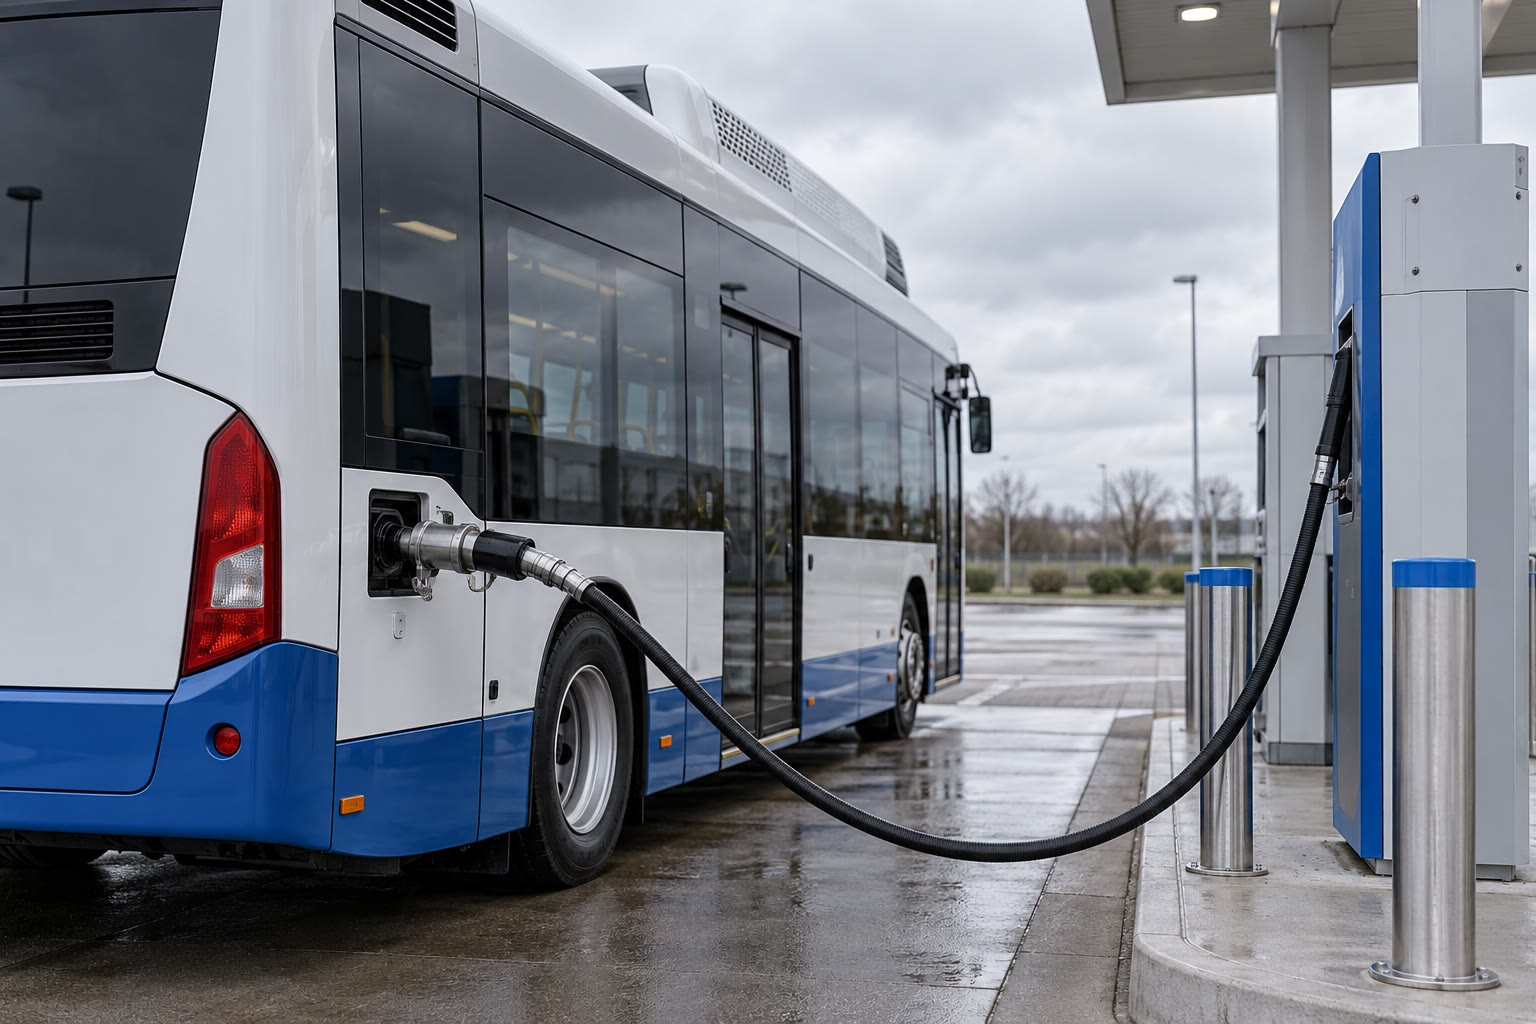
\includegraphics[width=0.5\linewidth]{images/book1/ai/g11-hydrogen-bus.jpg}

{\small A bus at a hydrogen station: its \omterm{def:g4:what-a-fire-needs:fuel}{fuel} releases only water.}
\end{omfigure}

\begin{safety}{\ghs[0.82cm]{GHS02}\ghs[0.82cm]{GHS07}}
% ledger: ghs:ethanol
Ethanol is highly flammable and irritating to the eyes. A spirit burner
is filled away from any flame, never refilled while hot, and used by the
teacher on a heat-proof mat.
\end{safety}

\section{Exercises}


\begin{exercise}[$\star$]\label{exo:g11:reaction-energy:1}
\omterm{def:g11:reaction-energy:exothermic}{Exothermic} or \omterm{def:g11:reaction-energy:exothermic}{endothermic}: wood \omterm{def:g4:what-a-fire-needs:burning}{burning}; ice melting; a cold pack being
squeezed; a hand warmer heating up; a green leaf making sugar in
sunlight?
\end{exercise}

\begin{exercise}[$\star$]\label{exo:g11:reaction-energy:2}
% ledger: dch:CH4
What energy does the \omterm{def:g8:combustion-and-fuels:complete}{complete combustion} of \qty{3.0}{mol} of methane
release?
\end{exercise}

\begin{exercise}[$\star$]\label{exo:g11:reaction-energy:3}
On the energy diagram of an \omterm{def:g11:reaction-energy:exothermic}{exothermic} reaction, which holds more
energy, the \omterm{def:g7:chemical-reactions:reactant}{reactants} or the products? Where does the difference go?
\end{exercise}

\begin{exercise}[$\star$]\label{exo:g11:reaction-energy:4}
% ledger: dch:C2H5OH
What energy does the \omterm{def:g8:combustion-and-fuels:complete}{complete combustion} of \qty{100}{g} of ethanol
release?
\end{exercise}

\begin{exercise}[$\star$]\label{exo:g11:reaction-energy:5}
What is a \omterm{def:g11:reaction-energy:bond-energy}{bond energy}? Why does breaking a bond always cost energy?
\end{exercise}

\begin{exercise}[$\star\star$]\label{exo:g11:reaction-energy:6}
Estimate, with bond energies, the energy of the reaction
\ce{2H2 + O2 -> 2H2O}, all gases. Is it \omterm{def:g11:reaction-energy:exothermic}{exothermic}?
\end{exercise}

\begin{exercise}[$\star\star$]\label{exo:g11:reaction-energy:7}
Estimate the energy of the \omterm{def:g4:what-a-fire-needs:burning}{combustion} of ethanol, \ce{C2H5OH + 3O2 ->
2CO2 + 3H2O}, with bond energies (draw the \omterm{def:g10:lewis-and-shape:lewis-structure}{Lewis structure} of ethanol
first), and compare with the measured \qty{1367.6}{kJ/mol}.
\end{exercise}

\begin{exercise}[$\star\star$]\label{exo:g11:reaction-energy:8}
% ledger: dch:C3H8, dch:CH4
Compute the energy released per kilogram of propane
(\qty{2219.2}{kJ/mol}) and of methane. Compare with the bar chart.
\end{exercise}

\begin{exercise}[$\star\star$]\label{exo:g11:reaction-energy:9}
% ledger: cp:water, dch:CH4
A gas cooker heats \qty{1.50}{L} of water (\qty{1500}{g}) from
\qty{15}{\celsius} to \qty{100}{\celsius}. What energy does the water
receive? What mass of methane is burnt if all the energy reached the
water? If only half of it did?
\end{exercise}

\begin{exercise}[$\star\star$]\label{exo:g11:reaction-energy:10}
Using the bar chart, rank the \omterm{def:g4:what-a-fire-needs:fuel}{fuels} by energy per kilogram. What mass of
hydrogen gives the same energy as \qty{1.0}{kg} of octane?
\end{exercise}

\begin{exercise}[$\star\star$]\label{exo:g11:reaction-energy:11}
Estimate the energy of \ce{N2 + 3H2 -> 2NH3}, all gases. \omterm{def:g11:reaction-energy:exothermic}{Exothermic} or
\omterm{def:g11:reaction-energy:exothermic}{endothermic}?
\end{exercise}

\begin{exercise}[$\star\star\star$]\label{exo:g11:reaction-energy:12}
% ledger: cp:water, dch:C2H5OH
In a spirit-burner experiment, \qty{250}{g} of water warm by
\qty{20}{\celsius} while \qty{1.20}{g} of ethanol burn. Compute the
energy received by the water, the energy the ethanol could release, and
the efficiency of the heating. Name three causes of the losses.
\end{exercise}

\begin{exercise}[$\star\star\star$]\label{exo:g11:reaction-energy:13}
% ledger: dfh:C8H18, dfh:CO2, dfh:H2O-l, dch:C3H8
Octane releases \qty{5470}{kJ/mol} and propane \qty{2219.2}{kJ/mol}.
Write their \omterm{def:g4:what-a-fire-needs:burning}{combustion} equations and compute the mass of carbon dioxide
each releases per megajoule. Compare with methane, \qty{49.4}{g}.
\end{exercise}

\begin{exercise}[$\star\star\star$]\label{exo:g11:reaction-energy:14}
For both methane and ethanol, the bond-energy estimate is smaller than
the measured energy released. Give the reasons, and explain why the
estimate is still useful.
\end{exercise}

\begin{exercise}[$\star\star\star$]\label{exo:g11:reaction-energy:15}
Estimate the energy of \ce{2H2O -> 2H2 + O2}, all gases. Why must energy
be supplied (for example as electricity) to make hydrogen from water?
Explain why hydrogen is called a way of \emph{storing} energy rather than
a source of energy.
\end{exercise}

\section{Problem: Which Fuel for the City Bus?}

\begin{problem}[{Weekend problem --- methane, ethanol, octane or hydrogen:
which gives the most energy per kilogram, and how much carbon dioxide per
megajoule?}]
\label{pb:g11:reaction-energy:1}
% ledger: dch:CH4, dch:C2H5OH, dfh:C8H18, dfh:CO2, dfh:H2O-l, be:C-H, be:OO-double, be:CO-double, be:O-H
A city compares four \omterm{def:g4:what-a-fire-needs:fuel}{fuels} for its buses: methane (natural gas), ethanol,
octane (for petrol) and hydrogen. The energies released by the \omterm{def:g8:combustion-and-fuels:complete}{complete
combustion} of one \omterm{def:g10:the-mole:amount}{mole} are: methane \qty{890.7}{kJ}, ethanol
\qty{1367.6}{kJ}, octane \qty{5470}{kJ}, hydrogen \qty{285.8}{kJ}, the
water being formed liquid.

\medskip
\noindent\textbf{Part I --- \omterm{def:g4:what-a-fire-needs:burning}{Combustion} equations.}
\begin{enumerate}
  \item Write the equation of the \omterm{def:g8:combustion-and-fuels:complete}{complete combustion} of methane.
  \item Of ethanol, \ce{C2H6O}.
  \item Of octane, \ce{C8H18}.
  \item Of hydrogen.
  \item Which \omterm{def:g4:what-a-fire-needs:fuel}{fuel} releases no carbon dioxide?
\end{enumerate}

\medskip
\noindent\textbf{Part II --- Energy per kilogram.}
\begin{enumerate}[resume]
  \item Compute the molar masses of the four \omterm{def:g4:what-a-fire-needs:fuel}{fuels}.
  \item Compute the energy released per kilogram for each, in
        \si{MJ/kg}.
  \item Rank the \omterm{def:g4:what-a-fire-needs:fuel}{fuels}.
  \item Hydrogen wins by far. Why is it still difficult to carry on a
        bus? (Think of its state at room temperature.)
\end{enumerate}

\medskip
\noindent\textbf{Part III --- Estimating with bond energies.}
\begin{enumerate}[resume]
  \item Draw the \omterm{def:g10:lewis-and-shape:lewis-structure}{Lewis structures} of the \omterm{def:g7:atoms-and-molecules:molecule}{molecules} of the \omterm{def:g4:what-a-fire-needs:burning}{combustion} of
        methane, and count the bonds broken and formed.
  \item Compute the energy needed to break the bonds.
  \item Compute the energy released by forming the new bonds.
  \item Deduce the estimate of $E_r$, and compare with the measured
        value: relative difference?
  \item Give two reasons for the difference.
\end{enumerate}

\medskip
\noindent\textbf{Part IV --- Carbon dioxide per megajoule.}
\begin{enumerate}[resume]
  \item What amount of methane must burn to release \qty{1}{MJ}?
  \item What mass of carbon dioxide does it release?
  \item Same question for ethanol and octane.
  \item Which carbon \omterm{def:g4:what-a-fire-needs:fuel}{fuel} releases the least carbon dioxide for the same
        energy? Why (compare the numbers of C and H \omterm{def:g7:atoms-and-molecules:atom}{atoms})?
  \item Hydrogen releases none when it burns. On what does its true
        benefit for the climate depend?
  \item State the final answer: what mass of carbon dioxide does methane
        release per megajoule?
\end{enumerate}
\end{problem}
